\section{Fuentes de señal auxiliares}
\label{sec:fuentes_auxiliares}

Además de las cuatro fuentes de cámara, el sistema incorpora varias fuentes de señal
auxiliares que permiten gestionar el estado de la emisión en momentos en los que la
mezcla principal no debe ser visible para el espectador, así como una entrada de audio
independiente para música de fondo.

\subsection{Fuente break e intro}

\texttt{break} e \texttt{intro} son fuentes de vídeo pregrabadas que el núcleo trata
exactamente igual que una cámara adicional: se conectan a los puertos 10004 y 10005
respectivamente mediante procesos FFmpeg, y aparecen en el mezclador como dos entradas
más. Sin embargo, dado que no aportan información relevante al realizador durante la
producción en directo, se ha optado por ocultarlas en la interfaz gráfica, manteniendo
su funcionalidad completa en el núcleo sin ocupar espacio en el panel de previsualizaciones.

\begin{itemize}
  \item \textbf{break}: vídeo en bucle empleado como pantalla de pausa animada durante
  los descansos del evento. FFmpeg lo envía con la opción \texttt{-stream\_loop -1}
  para que la fuente nunca quede en negro, independientemente de la duración del
  archivo. El realizador puede seleccionarlo directamente como fuente activa del
  mezclador, igual que las cámaras 1 a 4.
  \item \textbf{intro}: vídeo introductorio que se reproduce al inicio del evento o
  entre sesiones. A diferencia del break, la intro \emph{no} se reproduce en bucle
  continuo, sino que se dispara una sola vez cuando el realizador selecciona esa fuente
  en la interfaz gráfica.
\end{itemize}

\subsubsection{Mecanismo de disparo de la intro (\textit{vigilante})}

El comportamiento de disparo único de la intro plantea un reto arquitectónico: la GUI
de voctogui no puede ejecutar comandos externos sin bloquear el hilo principal de GTK.
Para resolverlo sin modificar el núcleo del sistema, se implementó un proceso
independiente denominado \texttt{vigilante\_intro.py}.

Este script actúa como un cliente silencioso del puerto de control TCP (9999): escucha
el flujo de notificaciones de estado que voctocore difunde por \textit{broadcast} y,
cuando detecta el mensaje \texttt{video\_status intro} (el realizador ha seleccionado
la fuente intro), ejecuta inmediatamente el script \texttt{lanzar\_intro.sh} mediante
\texttt{subprocess.Popen} sin buffering para garantizar una reacción instantánea.

Esta arquitectura sigue la filosofía de separación de responsabilidades de Voctomix:
el núcleo solo sabe mezclar señales; los automatismos de producción se implementan
como clientes externos que reaccionan a su protocolo de estado. Si el vigilante fallara,
el sistema de mezcla continuaría operando con plena normalidad.

\subsection{Entrada de audio}

El sistema incorpora una entrada de audio independiente en el puerto 18000, pensada
para inyectar música de fondo durante los estados de pausa o fuera de emisión. Esta
entrada acepta un flujo Matroska de sólo audio (PCM S16LE, 48~kHz, estéreo) y su
nivel de salida puede controlarse desde el protocolo de control.

\subsection{Stream Blanker: estados de emisión}

El stream blanker es el mecanismo que permite interrumpir la señal de programa hacia el
exterior sin interrumpir el flujo de trabajo interno del realizador. Se implementa en
\texttt{voctocore/lib/streamblanker.py} como un elemento GStreamer adicional interpuesto
entre la mezcla y el puerto de salida de streaming (puerto 15000).

El sistema define tres estados de emisión, controlables desde la barra de herramientas
de voctogui:

\begin{itemize}
  \item \textbf{LIVE:} se emite la mezcla activa producida por voctocore. El realizador
        controla en todo momento lo que ve el espectador.
  \item \textbf{PAUSE:} se emite el vídeo de pausa procedente del puerto 17000,
        acompañado de la música de fondo del puerto 18000.
        Se usa durante los descansos del evento para que los espectadores vean una pantalla
        animada mientras el equipo de producción prepara la siguiente sesión.
  \item \textbf{NOSTREAM:} se emite un vídeo de ``fuera de emisión'' procedente del
        puerto 17001, indicando al espectador
        que la transmisión ha finalizado o aún no ha comenzado.
\end{itemize}

El cambio entre estados se aplica sobre la señal de salida.
Desde la interfaz gráfica, el realizador dispone de tres botones (LIVE, PAUSE,
NOSTREAM) en la barra de herramientas.

La figura~\ref{fig:streamblanker_estados} muestra la interfaz del realizador y la
señal vista por el espectador en los estados NOSTREAM y PAUSE.

\begin{figure}[H]
  \centering
  % ── Columna izquierda: NOSTREAM ──────────────────────────────────────
  \begin{minipage}[t]{0.47\textwidth}
    \subcaptionbox{GUI en estado NOSTREAM.\label{fig:gui_nostream}}{%
      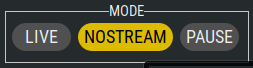
\includegraphics[width=\textwidth]{figuras/gui_nostream.png}}
    \par\vspace{0.3cm}
    \subcaptionbox{Señal del espectador en NOSTREAM.\label{fig:port_nostream}}{%
      \fbox{\begin{minipage}{\textwidth}\centering\vspace{1.0cm}
        \textit{[IMAGEN PENDIENTE]}\\[2pt]
        \texttt{figuras/port\_15000\_nostream.png}
        \vspace{1.0cm}
      \end{minipage}}}
  \end{minipage}
  \hfill
  % ── Columna derecha: PAUSE ───────────────────────────────────────────
  \begin{minipage}[t]{0.47\textwidth}
    \subcaptionbox{GUI en estado PAUSE.\label{fig:gui_pause}}{%
      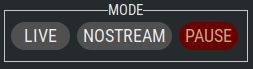
\includegraphics[width=\textwidth]{figuras/gui_pause.png}}
    \par\vspace{0.3cm}
    \subcaptionbox{Señal del espectador en PAUSE.\label{fig:port_pause}}{%
      \fbox{\begin{minipage}{\textwidth}\centering\vspace{1.0cm}
        \textit{[IMAGEN PENDIENTE]}\\[2pt]
        \texttt{figuras/port\_15000\_pause.png}
        \vspace{1.0cm}
      \end{minipage}}}
  \end{minipage}
  \caption{Estados NOSTREAM y PAUSE del stream blanker: vista del realizador (arriba)
           y señal recibida por el espectador (abajo).}
  \label{fig:streamblanker_estados}
\end{figure}
%   \label{fig:fsm_stream_blanker}
% \end{figure}
